\chapter{Evaluation} \label{chap:evaluation}

The evaluation of this work is divided into two parts. First, there will be a short summary of the observations that could be made after the previously mentioned run of the training pipeline was executed. In the second subchapter, the implemented top-k retrieval system will be evaluated using different methods. Here, the effects of the integrated top-k algorithms will be examined first and compared to one another. By doing that, both the number of accesses to the sorted lists as introduced in \autoref{chap:relatedwork}, as well as the runtime of the algorithms, will be analyzed. Afterward, an evaluation of the impacts of resource-aware model sets on the network utilization will be made.
  
  
  
  \section{Training Pipeline}
  
  Upon execution of the training pipeline runs that were introduced in the previous chapter, several different observations could be made. The following analysis of the models that were created in the previously mentioned training pipeline runs will be done for all created models – models that were created in the first as well as in the second run. Therefore, observations about models with window sizes of 1, 5, 10, 30, and 60 minutes will be made. Additionally, the performance metrics of models that use the concept of prediction horizons will be analyzed together with models that use the previously introduced 24 hour-shift or no future prediction aspect at all.

  In total, $23042$ models were created using the implemented training pipeline. With over $11$ hours, training the models with a window size of 1 minute took by far the longest time. Regarding the classifiers, training Random Forest models used up the most time during building, with an estimated average of about 30 seconds per model. In total, the training pipeline was running approximately for $29$ hours. Out of all models, $2632$ models have an accuracy of $0\%$. The total accuracy distribution of all created models can be seen in \autoref{fig:totalmodels}, which uses a logarithmic scale for better visibility. Following, almost $13\%$ of all trained models have an accuracy of $0\%$ and are therefore useless for further usage. The majority of the models with zero accuracy can be explained through the feature \texttt{previousOccupancy}: Out of all models with $0\%$ accuracy, $81\%$ (in absolute numbers $2130$) are missing \texttt{previousOccupancy} as a feature. The impact of \texttt{previousOccupancy} can also be seen in \autoref{fig:groupedprevocc}, which shows a grouped bar chart for models with and without \texttt{previousOccupancy} binned in $5\%$ steps.

  \begin{figure}[htbp]
    \centering
    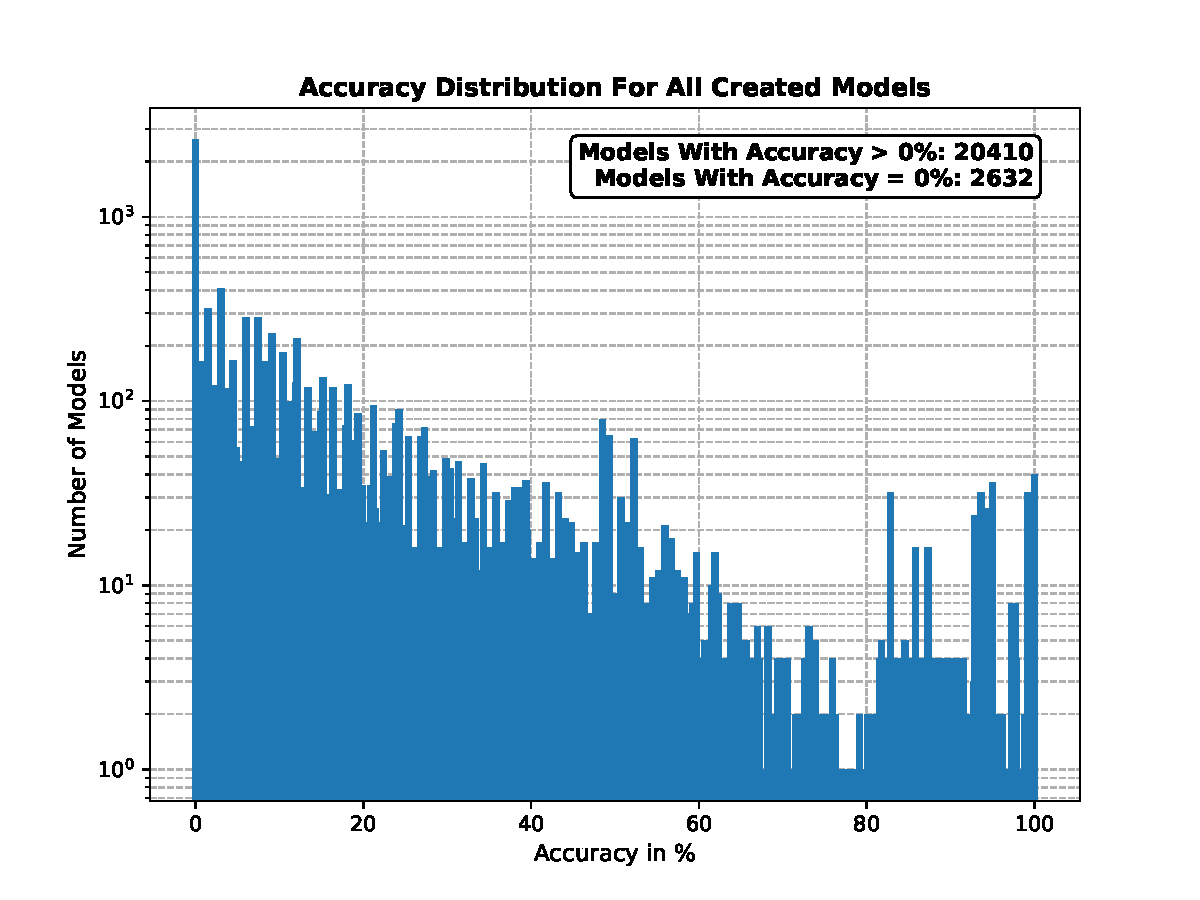
\includegraphics[height=10cm]{plots/totalmodels.pdf}
    \caption{Accuracy Distribution for All Created Models on a Logarithmic Scale}
    \label{fig:totalmodels}
  \end{figure}
  
  To expand on the findings from \autoref{fig:groupedprevocc}, it should be noted that out of all trained and stored models with an accuracy of over $90\%$, $346$ use \texttt{previousOccupancy}, and only $20$ don't. However, $18$ out of those $20$ models allegedly have an accuracy of $100\%$, which with a high probability makes them candidates for overfitting. This speaks for the indispensability of using the occupancy of the previous time slot as a feature when training a new model. Models that don't have access to this information seem to perform worse overall. When looking at this finding from a theoretical perspective, it should not be hard to see the reason for this behavior: In between two consecutive time slots (may it be one minute, or even 60 minutes), the occupancy of a specific parking lot usually should not change too much. Of course, a considerable change in occupancy during rush hours in the early morning or afternoon hours would be not surprising. However, this volatility in occupied parking spaces would most likely not happen rapidly in a matter of a few minutes, but rather in longer time periods, like a few hours. It therefore does not come as a surprise, that \texttt{previousOccupancy} plays such an important role in a model's performance.

 

  \begin{figure}[htbp]
    \centering
    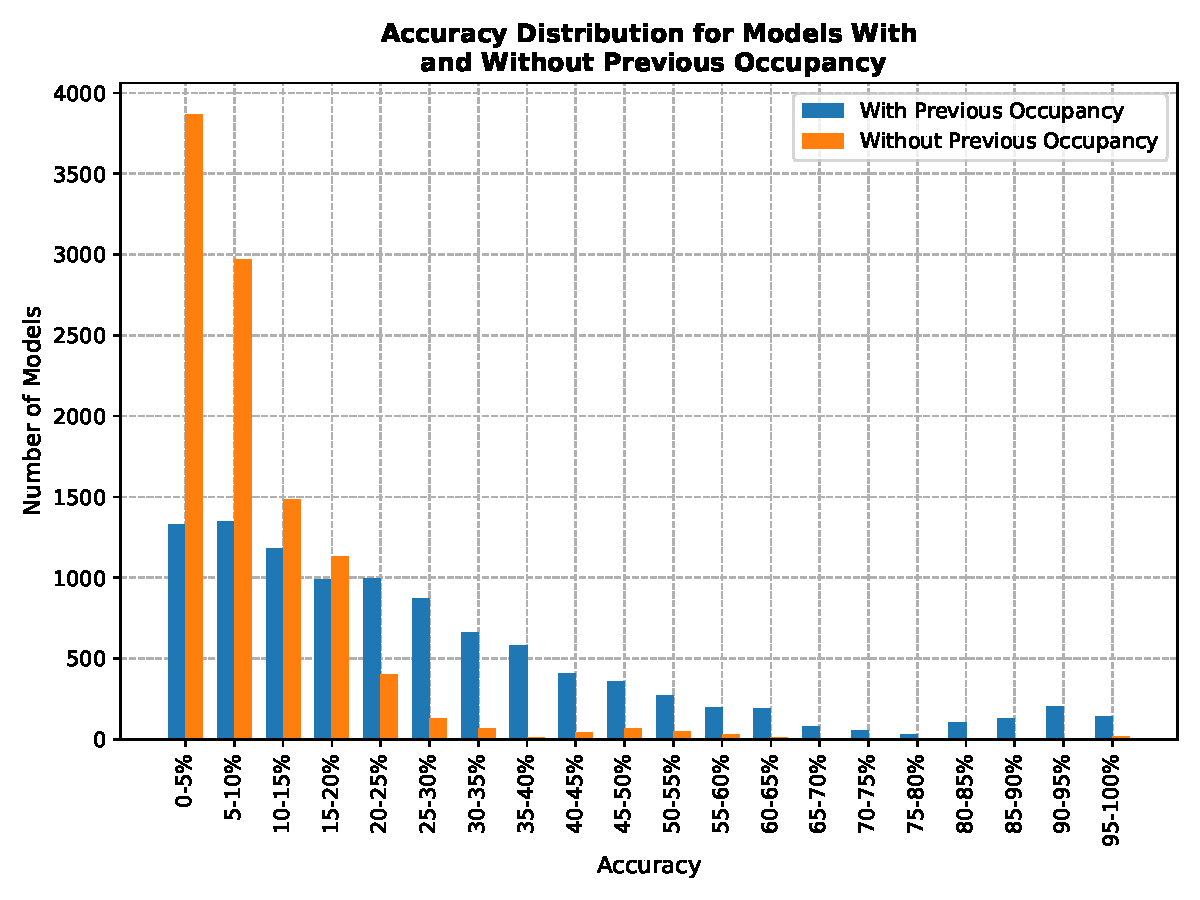
\includegraphics[height=10cm]{plots/grouped_prevocc.pdf}
    \caption{Accuracy Distribution for Models With and Without Previous Occupancy}
    \label{fig:groupedprevocc}
  \end{figure}


  
  Another thing that became apparent when looking at the created models, was that small variations in certain metrics could make big differences in performance. One of the biggest influences comes from the window size of a model: a fine-grained segmentation mostly means an increase in performance metrics like accuracy, compared to a coarse-grained segmentation. Small window sizes for models using the implemented functionalities of the \texttt{predictionHorizon} are always performing better, than big window sizes for models that make use of \texttt{predictionHorizon}. This observation holds for models using the 24 hour-shift and models with no future prediction aspects. However, the accuracy for models with neither \texttt{predictionHorizon} nor 24 hour-shift tends to be higher than for models that use some form of future prediction: In total, $2,8\%$ of the models that use no form of future prediction (i.e. predict the same time slot as they are executed in) have an accuracy value of over $90\%$, while the same is true for only $0,9\%$ of models that make use of a prediction horizon. This behavior can be seen in \autoref{fig:nofuture} and \autoref{fig:predhor}. The highest accuracy value for a model that was trained using a 24 hour-shift only reached an accuracy of 67\%. In general, the distribution for models using a 24 hour-shift tends to be skewed towards lower accuracy values, as shown in \autoref{fig:shift24h}. Note, that in \autoref{fig:nofuture}, \autoref{fig:predhor}, and \autoref{fig:shift24h} models with an accuracy value of 0\% are disregarded to provide a better visualization of the accuracy distribution.
  
  \begin{figure}[htbp]
    \centering
    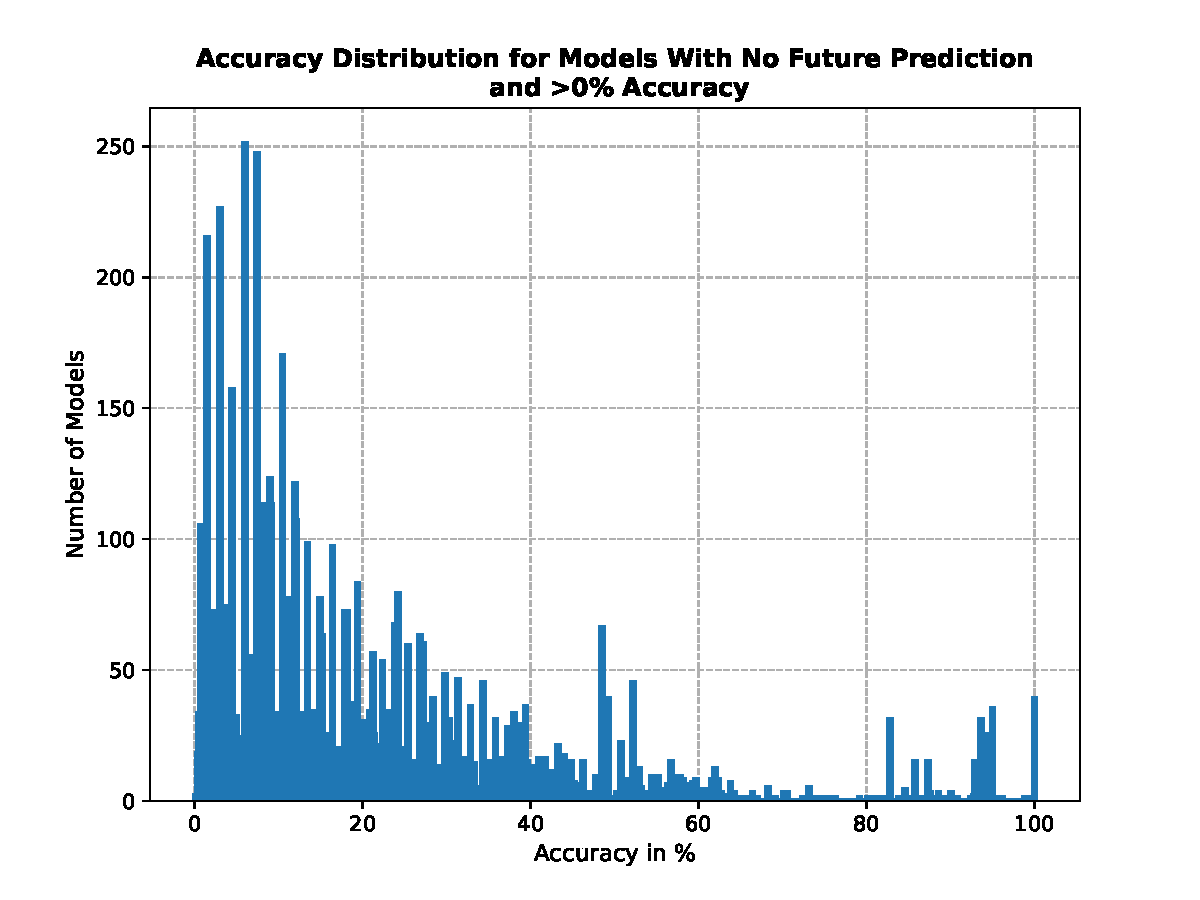
\includegraphics[height=10cm]{plots/nofuture.pdf}
    \caption{Accuracy Distribution for Models With No Future Prediction and >0\% Accuracy}
    \label{fig:nofuture}
  \end{figure}

  \begin{figure}[htbp]
    \centering
    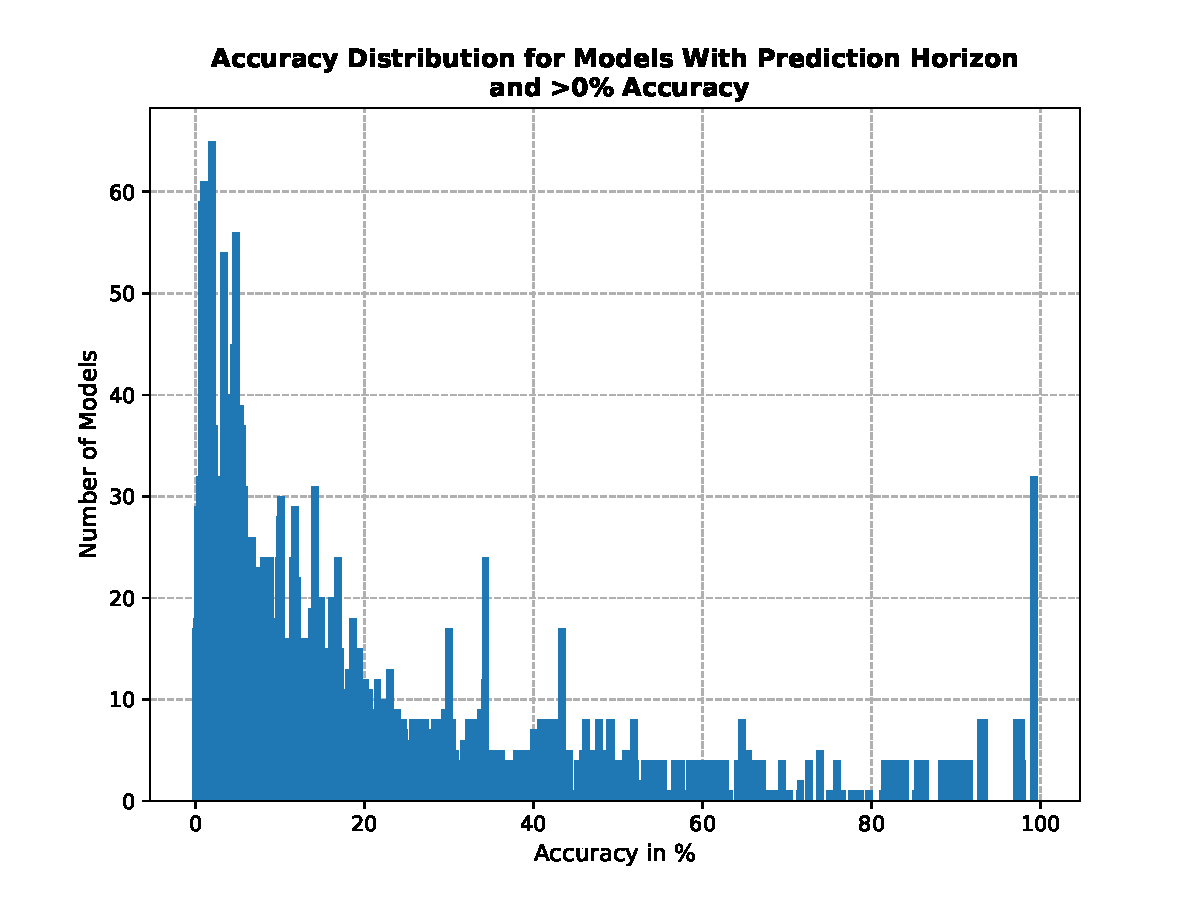
\includegraphics[height=10cm]{plots/predhor.pdf}
    \caption{Accuracy Distribution for Models With Prediction Horizon and >0\% Accuracy}
    \label{fig:predhor}
  \end{figure}

  \begin{figure}[htbp]
    \centering
    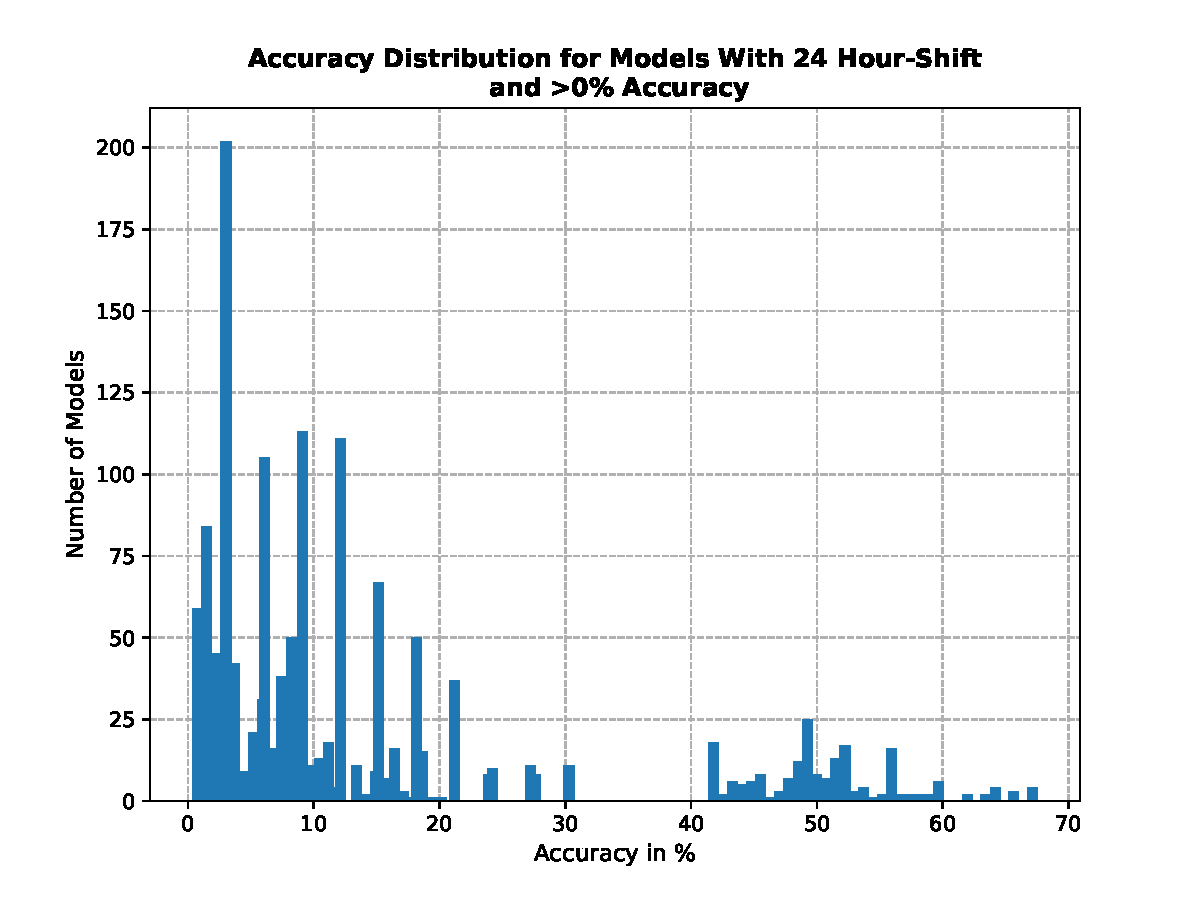
\includegraphics[height=10cm]{plots/shift24h.pdf}
    \caption{Accuracy Distribution for Models With 24 Hour-Shift
    and >0\% Accuracy}
    \label{fig:shift24h}
  \end{figure}


  The reason for these observations seems straightforward, considering the models with future prediction (i.e. models using either a 24 hour-shift or a \texttt{predictionHorizon}) have to consider much more uncertainties in the regression, than models that just predict the occupancy for the current time slot. The fact that models that were implemented using the concept \texttt{predictionHorizon} seem to predict future occupancy values better than models using the 24 hour-shift can be traced back to the values the \texttt{predictionHorizon} assumes for the created models: These models predict the occupancy value in 60 minutes at most. From \autoref{fig:predhor} and \autoref{fig:shift24h} it can therefore be concluded, that models have less trouble predicting for relatively shorter time intervals, than for 24 hours.
  
  Another observation that was made, is that feature scaling seemed to have close to no impact on the performance of the models. The vast majority of performance metrics (accuracy, MAE, MSE, RMSE) stay the same for a model compared to its feature-scaled pendant. However, as stated in \autoref{chap:implementation}, feature scaling was only done for some models. Further tests and evaluations using feature scaling on models with different window sizes and prediction horizons could produce unexpected new insights.
  
  In summary, the observations that could be made when looking at the performance metrics of the models trained by the constructed pipeline are mostly in line with prior expectations. The time difference between the inference of the model and the time that is to be predicted as well as the feature \texttt{previousOccupancy} rightfully have a large influence on a model's performance. The lack of impact of feature-scaled models is something to further research and analyze.
  
  
  
  \section{Retrieval System}

To evaluate whether the previously introduced top-k algorithms perform any better than a simple-to-implement NA, various tests have been performed to show both time consumption as well as sorted and random accesses of all implemented top-k algorithms. In order to assess the necessary data about time consumption and computational resources used, the implementation of the algorithm has been changed slightly. Counters were added that would increment every time a sorted access or a random access was made. In addition, the Python standard module \texttt{time} was used to create time stamps at the beginning and end of each operating algorithm in order to exactly measure the time, each algorithm execution takes. 
% Both accesses and time consumption have been measured separately for every algorithm round. Consequently, if an API call contains three different prediction horizons, in total four execution times are measured: One for each prediction horizon and one for the second round of top-k algorithms which selects the best model sets out of the created combinations. 
To give insight into how the data for the evaluation was gathered, the used settings for the API calls are displayed along with the corresponding observations. 



\subsection{Accesses}

Before comparing the number of accesses across the different kinds of top-k algorithms, first, it had to be made sure that inside each algorithm the number of accesses stayed the same, which was previously not the case. The reason for this was that the lists that were handed over to the top-k algorithm were sorted in an arbitrary way when dealing with the same values. For example, all models having 3 features were sorted differently in the list (while of course still being ranked after the models with 2 features, and before the models with 4 features). This results in varying favorability of processing which leads to different orders in each API call. Therefore, a second attribute has been added to the sorting function that is called when creating the different lists before executing the algorithms. It is therefore ensured, that when carrying out the same API call multiple times, all items contained in the lists (models in round one, or model sets in round two) are always in the exact same order, even when having to deal with ties. To eliminate this randomness and have the models be sorted in the exact same way, the model ID has been added as a second sorting attribute. Subsequently, the algorithm works deterministically, as the number of accesses stays the same for a predetermined request. 


% Models used for evaluating number of accesses
\begin{table}[htbp]
\centering
    \begin{tabular}{ l | c  c  c }
        \toprule
        &
\textbf{Request 1}      
& \textbf{Request 2}   
& \textbf{Request 3} \\\midrule

\textbf{pID} & 38 & 38 & 634 \\\midrule
\textbf{windowSize} & [1,5] & [1,5] & [1] \\\midrule
\textbf{perfMetric} & acc & rmse & acc \\\midrule
\textbf{k1} & 8 & 6 &10 \\\midrule
\textbf{k2} & 3 & max & 10 \\\midrule
\textbf{predHor} & [10,30,60] & [10,60] & [10,30]\\\midrule
\textbf{perfWeight} & 0.8 & 0.78 & 1 \\\midrule
\textbf{AMSWeight} & 0.65 & 0.2 & 1\\\midrule
\textbf{algorithm}  & \multicolumn{3}{c}{NA, FA and TA for every request}  \\\midrule
\textbf{combineSameFeatures} & false & false & false \\\midrule
\textbf{calculateQSL} & min & avg & max\\
        \bottomrule
    \end{tabular}
\caption{Requests Used for Evaluating Number of Accesses} \label{accesses}
\end{table}

After the consistency of the number of accesses for an algorithm has been ensured, the actual evaluation could be started. To evaluate the number of accesses for each algorithm, three different exemplary requests have been created, as seen in \autoref{accesses}. The API calls were designed to represent a diverse spectrum of possible requests. Each request was then run for every algorithm each. As stated before, following Fagin’s reasoning, TA will in every case require less than or the same amount of sorted accesses as FA \cite{fagin2002}. This is indeed backed by the observed data: In every one of the three requests, TA required the least number of sorted accesses, followed by FA and NA, as seen in \autoref{fig:access}. Note, that because NA uses vastly more sorted accesses than FA or TA, the graph had to be displayed on a logarithmic scale to ensure clarity. 

In the first request, TA only used 0,4\% and FA only 1,1\% as many sorted accesses as NA used. In other words, TA and FA only had to iterate over around 1\% of the entire model list that was provided for that particular request. Out of all three requests, NA had the most accesses in Request 1 (namely 52240), because it is the only request that inquires three different prediction horizons, resulting in a total of 4 algorithm executions (one for each prediction horizon plus one for the actual model set retrieval). This behavior can also be inspected in Request 2 and 3, where TA uses only 0,7\% and 0,1\% and FA only 1,2\% and 2,0\% as many sorted accesses as NA respectively. The fact that NA uses by far the most sorted accesses out of the three algorithms should not come as a surprise, however, as NA only relies on sorted access (i.e. does not do any random accesses) and traverses through the entire model list before producing an output. Still, the dimension of the difference in sorted access becomes apparent when looking at the absolute numbers from the introduced exemplary requests. Across all algorithm rounds and requests, TA used a mean of 48,1 sorted accesses per algorithm call whilst this value is 132,7 for FA and 10222,4 for NA.

The computation advantage of FA and TA over naïvely iterating through the entire model/model set list is apparent. This observation however lacks informative value, as NA does not do any random accesses, that the other two algorithms heavily rely on. It might therefore be necessary to look at the number of total accesses per algorithm, by summing up both random and serial accesses. Doing this, TA uses a mean of 146,2 total accesses per algorithm call, followed by FA with 379,1 and NA with still 10222,4. Therefore, it can be seen that if even every form of access is considered, NA will still have significantly more accesses to do, in order to return the top-k results. 

\begin{figure}[htbp]
    \centering
    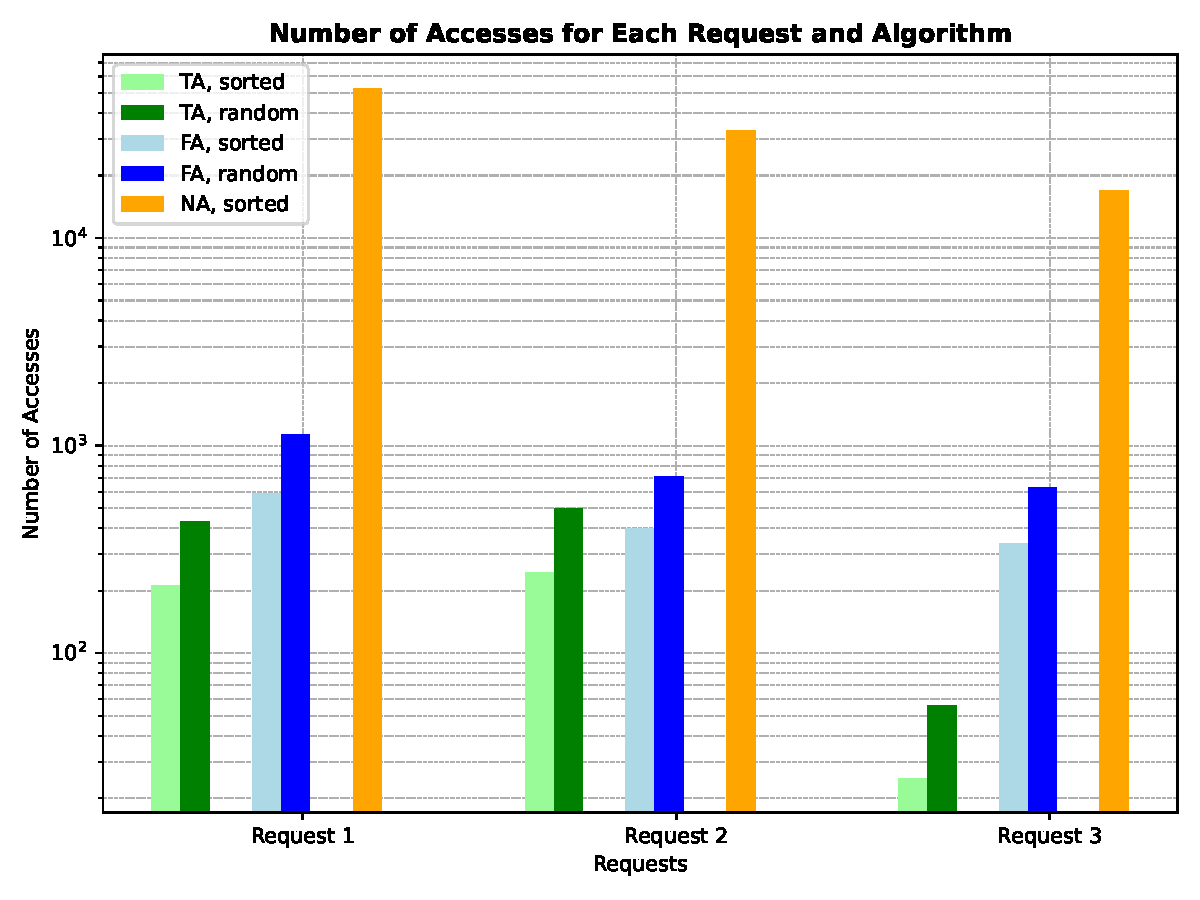
\includegraphics[height=10cm]{plots/grouped_accesses.pdf}
    \caption{Number of Accesses for Each Request and Algorithm on a Logarithmic Scale}
    \label{fig:access}
  \end{figure}


Regarding the number of random accesses, a comparison between TA and FA can be made. As TA in its design relies more heavily on random accesses than FA, the former was expected to have at least a similar number of random accesses than the latter. This is because, in TA, every accessed grade is instantly followed up by the randomly accessed missing grade of the same item. In FA, however, the seen objects are only randomly accessed at the end, when $k$ objects have been fully seen already. However, the average number of random accesses of 98,1 for TA and 246,4 for FA, came as a surprise. Apparently, TA still uses fewer random accesses than FA, which speaks for TA using less computational resources. Only in one occurrence did FA use fewer random accesses than TA: Getting the top $k$ model sets in the second request required not a single random access by FA, whilst requiring 44 by TA. This however is easily explained when looking at the specified \texttt{k2} in this request. Selecting \texttt{max} as \texttt{k2} results in an algorithm returning all items that are in the model set list. In the case of FA, this means the algorithm serial accesses every item in order and by the time the random access phase is started, the algorithm already has seen every object in its entirety. FA does therefore not have to do any random accesses. The biggest difference in the number of random accesses between TA and FA can be seen in Request 3: While TA uses 56, FA uses 625, which is over 11 times more random accesses. The reason for this could be a favorable distribution of models within the lists, for TA.

In summary, the expectations of both FA and TA have been fulfilled, as both top-k algorithms use significantly less accesses than a naïve approach of selecting the top-k elements. In addition, TA required fewer accesses than FA, making it the most access-friendly out of all three observed algorithms. 



\subsection{Execution Time}

After having assessed the number of accesses each algorithm has to do in order to return the top-k elements, the focus will now be the execution time of these algorithms. Here, it is important to not confuse the execution time of the model set retrieval process with the inference time of the models. The latter refers to the time a model takes between the model receiving an input and producing an output \cite{marco2019}. The execution, run, or retrieval time that will be analyzed in this chapter, however, addresses the aggregated time that passes between the calling of the algorithm function and returning its result for every algorithm call. 


Because of changes in local memory like cache and other simultaneous running programs, it is apparent that the execution time for each algorithm will at least slightly vary for each run. It is therefore necessary to run the respective requests for each algorithm multiple times and then take the average out of the observed execution times in order to make a fair and valid comparison. To get a better understanding of what processes take up the most time, the retrieval process was divided into smaller steps, each representing one or a group of similar relevant operations. When undergoing the first runs, using the same requests that were used for assessing the number of accesses, it became evident that there was little to no observable difference in run time between the three different algorithms - neither in total run time nor the time spent in \texttt{Algorithm round 1} and \texttt{Algorithm round 2}. At this time, 23.042 models were stored in the model database. Using the previously used Request 1 from \autoref{accesses} as an example, the difference in total execution time over all rounds (summing up the three prediction horizon rounds and the model set round) between the algorithms was not larger than 0,02 seconds. Time differences like this are too small to make any meaningful interpretations about the algorithms' runtime performance. To magnify the time differences and produce significant evaluation results it was then decided to add a much larger number of models to the model database so the top-k algorithms would have longer lists to work with. Using a for-loop in \texttt{postgreSQL}, exactly 200.000 instances of the same model were added to the model database, leading to a total of 223.042 models to consider. For the evaluation, it was sufficient to only add the metadata about the model, like window size and features, without having to add the actual model content as a byte array. \autoref{time} shows the subsequently created request that made the algorithms consider those newly added models. For this part of the evaluation, only one request was used to get data regarding the run time for each algorithm. The reason for this is that only a very specific type of model could be considered for this evaluation considering the additionally added 200.000 models all share the same parameters. To include those models in the retrieval execution, it had to be made sure that the request corresponds to those parameters. Therefore, a significant variation in the requests could have not been accomplished, resulting in only one request for the evaluation of execution time. In general, however, more different requests and therefore more different data sources would of course enrich the informative value of this evaluation.



% Models used for evaluating execution time
\begin{table}[h]
\centering
    \begin{tabular}{ l | c}
        \toprule
        &
\textbf{Request 1}      
 \\\midrule

\textbf{pID} & 634 \\\midrule
\textbf{windowSize} & [5] \\\midrule
\textbf{perfMetric} & acc  \\\midrule
\textbf{k1} & 3\\\midrule
\textbf{k2} & 5 \\\midrule
\textbf{predHor} & [30,60]\\\midrule
\textbf{perfWeight} & 0.75 \\\midrule
\textbf{AMSWeight} & 0.2\\\midrule
\textbf{algorithm}  & NA, FA and TA  \\\midrule
\textbf{combineSameFeatures} & false \\\midrule
\textbf{calculateQSL} & min \\
        \bottomrule
    \end{tabular}
\caption{Request Used for Evaluating Execution Time} \label{time}
\end{table}




As expected, the differences in runtime became apparent once a larger model database was used. The request shown in \autoref{time} was run 20 times per algorithm.  \autoref{fig:timenaive}, \autoref{fig:timefagin}, and \autoref{fig:timethreshold} show the developed steps and their corresponding mean execution time for every algorithm. The shown times are the mean values of all 20 executions for every algorithm and the graphs had to be put on a logarithmic scale, as certain steps in the retrieval process needed vastly more time to be finished than other steps. Looking at the total execution time, the data backs up what was to be expected: The request using TA finishes the fastest, with a mean total of around 40 seconds. FA finishes slightly slower with around 57 seconds and NA takes the longest execution time with about 68 seconds on average. Looking at the time spent on the actual top-k algorithms, it can be confirmed that NA in fact needs significantly more time iterating through the entire model list (\texttt{Algorithm round 1} in \autoref{fig:timenaive}) than FA or TA need to retrieve the top-k models by using sorted and random accesses (\autoref{fig:timefagin} and \autoref{fig:timethreshold}). The longer runtime of NA is explainable by its general procedure: Having to access every item in a list of over 200.000 items takes up much more time than only accessing the topmost items in each list. The runtime of \texttt{Algorithm round 2} shows no substantial difference between the three algorithms, which could be traced back to the considered lists being considerably smaller than the lists from the first algorithm round: As in the request used for this evaluation, \texttt{k} equals $3$, for every prediction horizon 3 models are retrieved in the first algorithm round, resulting in the creation of $3 \cdot{} 3 = 9$ model sets. Therefore, the list that the algorithms have to look through in \texttt{Algorithm round 2} is only of size 9, which apparently is too small for TA and FA to unfold their true potential. NA even is faster than the two sophisticated top-k algorithms in the second algorithm round, which might be due to an overhead of TA and FA.


\begin{figure}[htbp]
    \centering
    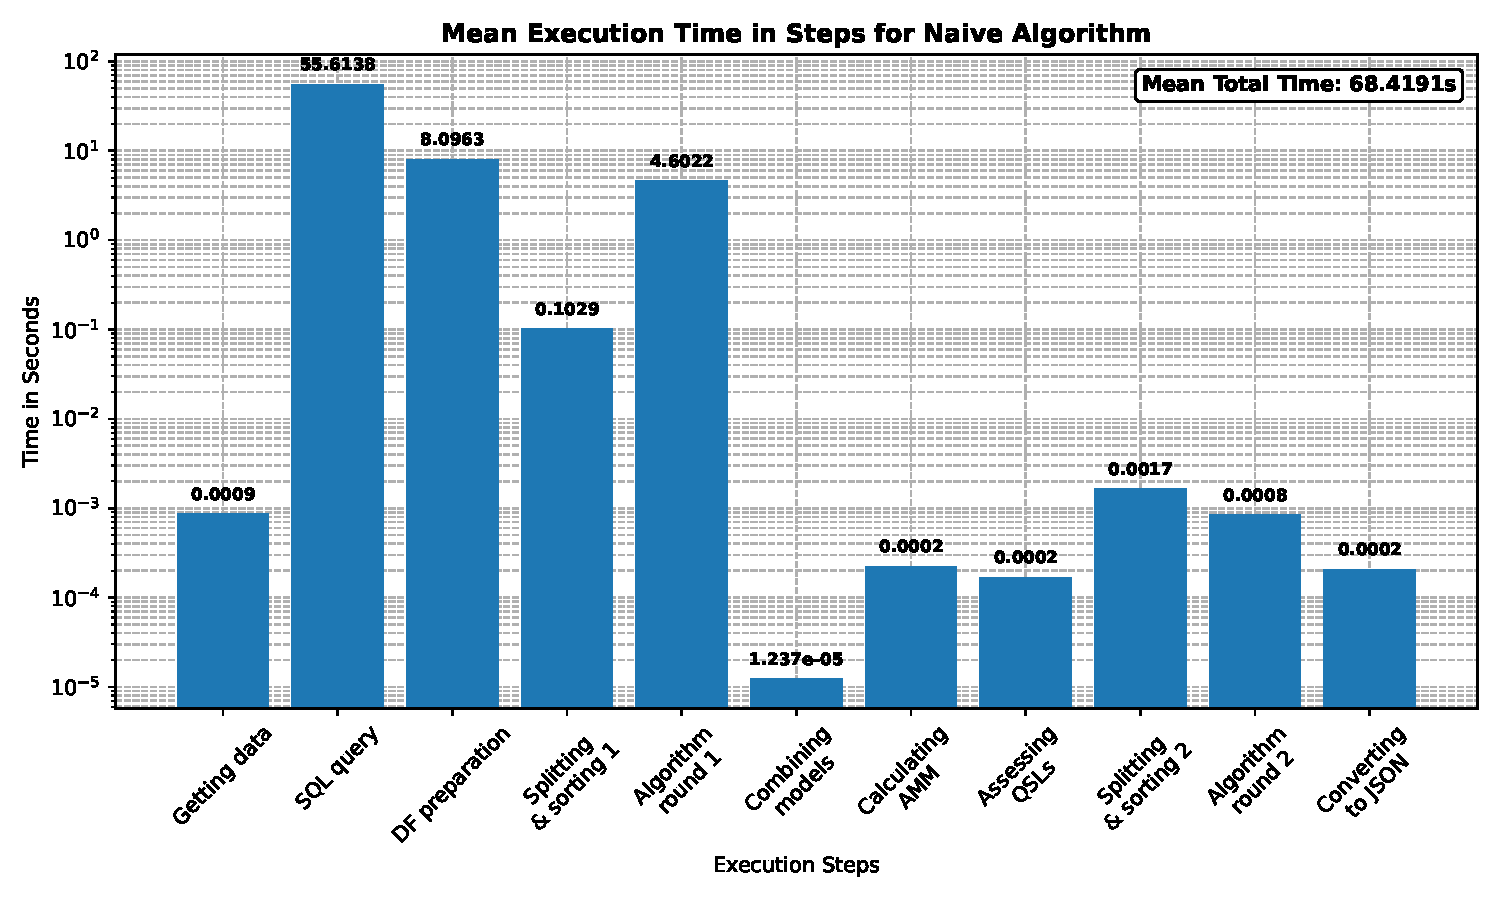
\includegraphics[height=9cm]{plots/executiontime_naive.pdf}
    \caption{Mean Execution Time in Steps for Naive Algorithm on a Logarithmic Scale}
    \label{fig:timenaive}
  \end{figure}

  \begin{figure}[htbp]
    \centering
    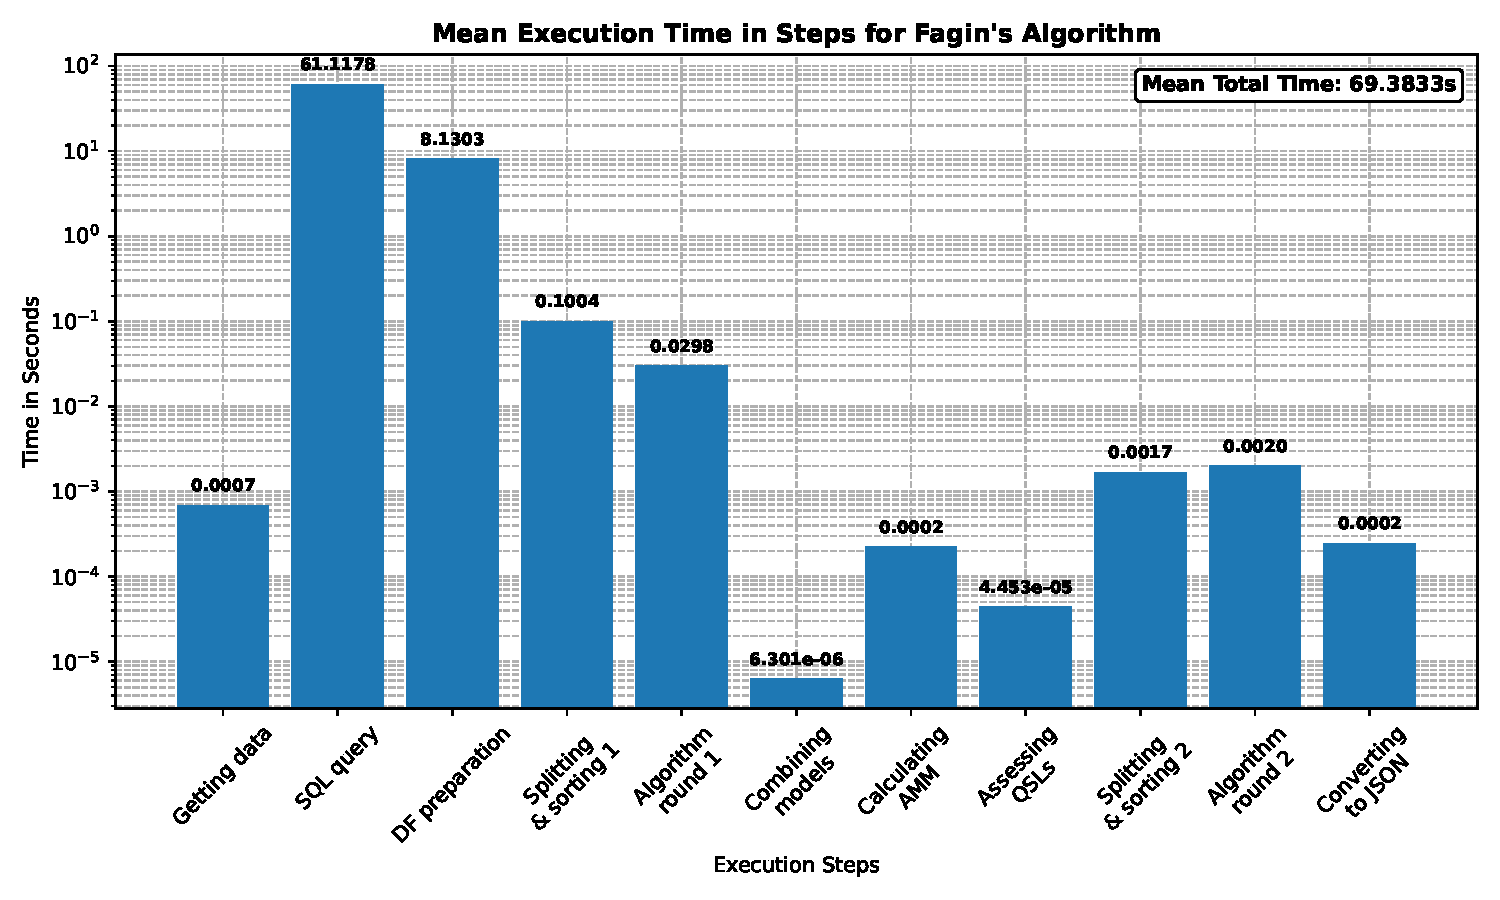
\includegraphics[height=9cm]{plots/executiontime_fagins.pdf}
    \caption{Mean Execution Time in Steps for Fagin's Algorithm on a Logarithmic Scale}
    \label{fig:timefagin}
  \end{figure}

  \begin{figure}[htbp]
    \centering
    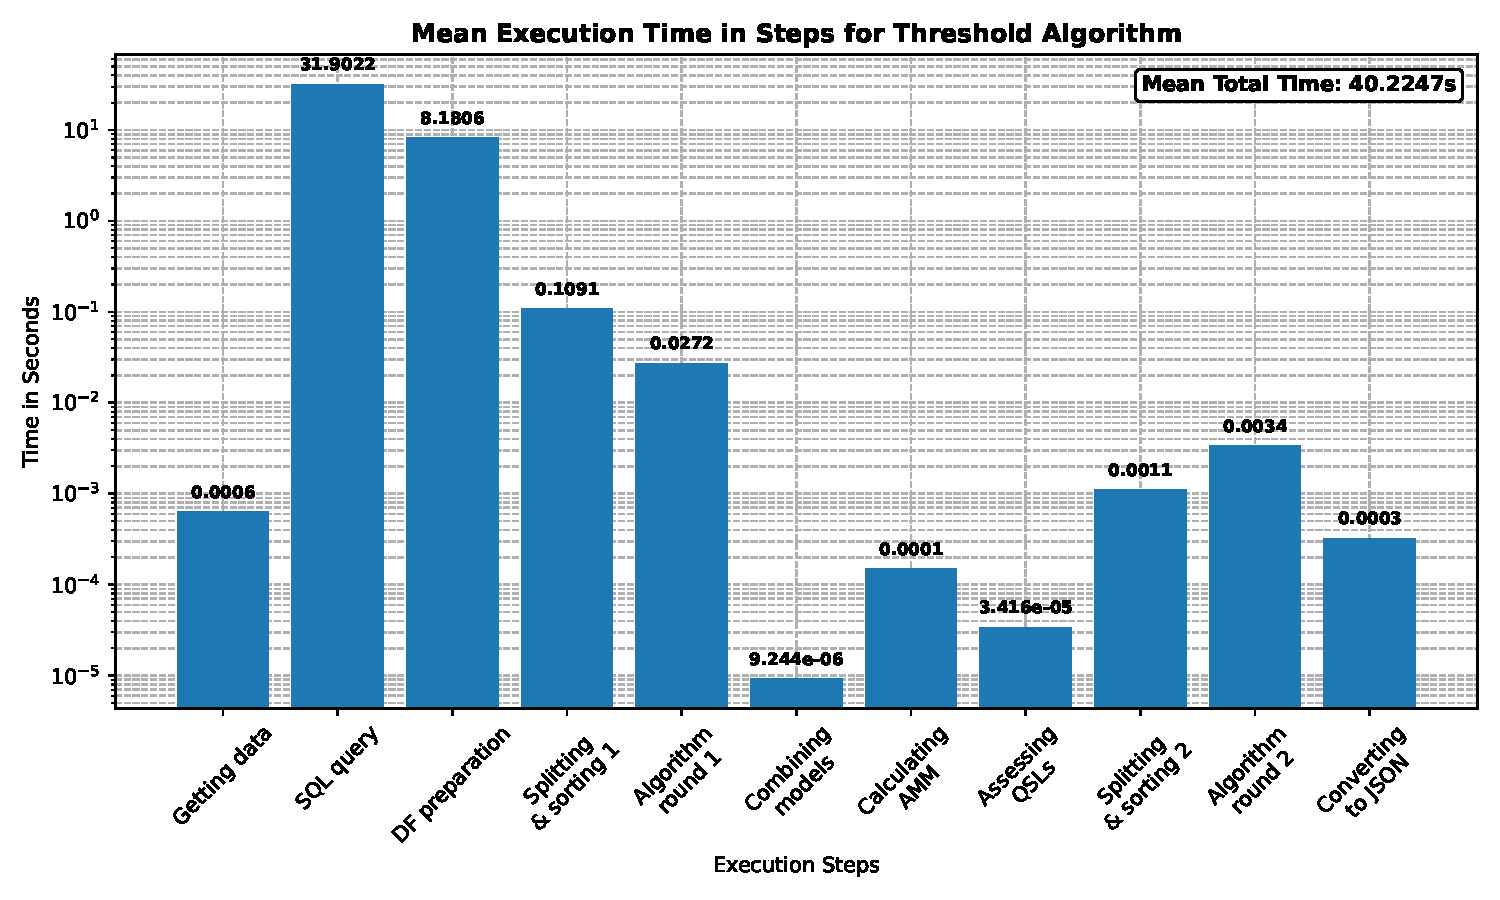
\includegraphics[height=9cm]{plots/executiontime_threshold.pdf}
    \caption{Mean Execution Time in Steps for Threshold Algorithm on a Logarithmic Scale}
    \label{fig:timethreshold}
  \end{figure}

Looking back at the mean total execution time, it becomes observable however, that the time difference of more than 11 seconds between NA and the other two algorithms can not be attributed to the different runtimes in \texttt{Algorithm round 1} only. The plots show, that the step \texttt{SQL query}, which represents the time it takes for preparing a SQL statement using the parameters from the request, executing the query, and storing the result in a \texttt{dataframe}, shows significantly different times for each algorithm. This step is by far the most time-consuming operation in the entire retrieval system, taking up on average 82\% of the entire retrieval process across all three algorithms. Because the retrieval process is the same no matter what algorithm is chosen, every step (excluding the algorithm runtime itself) should take up the same time. This can generally be affirmed by the observed data, with the exception of \texttt{SQL query}. Even though the same amount of data is queried from the model database for every algorithm, this step takes about 24 fewer seconds for the request using TA (31,9 seconds), than for the request using NA (55,6 seconds), as seen in \autoref{fig:timenaive} and \autoref{fig:timethreshold}. For FA, \texttt{SQL query} takes 48 seconds to complete, as seen in \autoref{fig:timefagin}. This behavior is hard to interpret, as in theory this step should need approximately the same time across all algorithms. It has to be assumed, that differences in CPU usage of the local machine or varying traffic in the \texttt{postgreSQL} database could be attributed to the unequal time consumption of \texttt{SQL query}. This shows, that further research is required to assess the total execution times per top-k algorithm in an unbiased way. 

Despite this falsification of the total execution time by the different values in the step \texttt{SQL query}, the algorithm execution time itself still behaves like expected: TA and FA perform best, as they make use of random accessing in addition to sorted accesses. However, as TA uses significantly less sorted and random accesses than FA (as seen in \autoref{fig:access}), it was expected to have a significantly shorter runtime than FA. The gathered data shows, that combining both algorithm rounds, TA is only 0,0002 seconds faster than FA, which is impossible to properly interpret. Nonetheless, the similarities in runtime of the two algorithms can be caused by a variety of reasons. For one, an algorithmic overhead can cause TA to run slightly slower than expected. This of course could as well be due to varying processes running in the background of the local machine. In addition, sections like calculating the threshold value of TA could potentially cause to add time to the execution that could then further be compensated by the saved time accomplished by the fewer number of accesses. Furthermore, the chosen data structures like \texttt{pandas} \texttt{dataframe} could very well be not the most efficient way to handle the processed data. It is possible that other data structures like lists could make it possible to save some more fractions of a hundredth of a second in execution time. However, it is not the aim of this work to micro-optimize the provided source code. 

Another aspect that was inspired by this evaluation, was the redundancy of the step \texttt{Splitting \& sorting 1} and \texttt{Splitting \& sorting 2} for NA. These steps describe the act of dividing the list of all models or model sets into two lists, consisting of one metric each (i.e. performance and resource awareness) and sorting each list in relation to that metric. As NA only works on one list, by iterating over it completely and calculating the score for every single item, the step that is responsible for creating the two lists and sorting them can be skipped for NA. However, in the current implementation, this optimization for NA is not yet done, making it an option for further work on this project. Another alternative could be to get rid of the splitting and sorting steps altogether, by working with pre-sorted lists for all requests. The retrieval system would then obtain the necessary, presorted lists corresponding to the requests' parameters. Deriving from the possible \texttt{pID}, \texttt{windowSize} and \texttt{predHor} values, subsequently $2 \cdot 2 \cdot 3 = 12$ different lists would have to be created and stored for access. If that expenditure is worth it to save the time on \texttt{Splitting \& sorting 1} and \texttt{Splitting \& sorting 2} is to be inspected further. Considering the splitting and sorting steps only take up about 0,1 seconds, these optimizations are not expected to have a significant change on the overall total retrieval time for any algorithm though. 

The evaluation of the implemented model set retrieval system shows that regarding execution time of the top-k algorithm, there is in fact a difference between a naïve approach and approaches that make use of random access. While these time differences might still seem marginal in relation to the total execution time, they might gain relevance once multiple queries are started after one another, or even a larger model database than the one utilized for evaluation is being used. Furthermore, this evaluation motivated conducting further research on the total execution time of each algorithm in a controlled, non-biased environment in order to get rid of possible conflicting variables, like current CPU usage.

  
  
\subsection{Network Utilization}


An analysis of the implications of using resource-aware model sets will finalize the evaluation of this project. Up to this point, the various options for creating model sets that make efficient resource utilization possible have been introduced and the decisions that lead to the current implementation have been explained. However, the final advantages of using resource-aware model sets are yet to be properly seen. This section aims to give an overview of the benefits resource-aware model sets can bring regarding data transmission. For this, a simple extrapolation will be made using the structure of the parking occupancy prediction use case as an example.

To show what implications the use of resource-aware model sets has, there are some assumptions to be made. It is assumed that in a running prediction system, if $m$ is the window size of a specific model, after $m$ minutes this model produces a new prediction. This means that not only does a model with a window size of 5 minutes segment the training data into slots of the size of 5 minutes, but also does this model predict the parking occupancy for the chosen prediction horizon every 5 minutes. This behavior is also the reason for penalizing models with a small window size by reducing their intra-model Resource Awareness Score as seen in \autoref{ras}: A small window size means more predictions which in turn require repetitious data transmissions. Another assumption is that features with more or less constant values like \texttt{year} or \texttt{month} have to be transmitted from the prediction system to the working model set for every prediction. In other words, there is no way for the model to directly access any time-specific features in order to save data transmission. Additionally, it is assumed that the datatypes and therefore the memory size of every feature is the same as they are stored in the preprocessed database. The reason for this presumption is, that it is likely that in a real-life scenario, accessing live data like temperature or humidity will require not only more time than getting other values but also more memory size than the single double value both temperature and humidity are stored as. For simplicity, this evaluation therefore assumes a predictable memory size for each feature. \autoref{datasizes} shows the data types used to store each feature and the resulting memory sizes. Lastly, one remark has to be made about the general architecture of the PAP use case: For this evaluation it has to be assumed, that PAP works as a distributed system, meaning that data has to be sent from the sensors to other nodes. In such a distributed system, many different edges exist, and the transfer of data is not limited to the data flow depicted in this section. The aggregation of attributes into features, as inspected in the following paragraphs, will therefore only portray a small part of the network utilization in the whole system. In addition, the following evaluation will generally be an underestimation, as the data transfer that is being sent in a real-life scenario is usually larger than what is being calculated theoretically. Nevertheless, the following assessment will still be a valid and precise estimation of the system's network utilization, as the features will use up a significant part of the bandwidth in a production setting \cite{sunkel2022}.


% Data types table
\begin{table}[h]
\centering
    \begin{tabular}{  l  l  l  l }
        \toprule
\textbf{Index}        
& \textbf{Feature}      
& \textbf{Data type}   
& \textbf{Memory size} \\\midrule

0 & temperature & double & 8 bytes \\\hline
1 & humidity & double & 8 bytes \\\hline
2 & weekday & integer & 4 bytes \\\hline
3 & month & integer & 4 bytes \\\hline
4 & year & integer & 4 bytes \\\hline
5 & timeslot & integer & 4 bytes \\\hline
6 & previous\char`_occupancy & double & 8 bytes \\

        \bottomrule
    \end{tabular}
\caption{Data Types and Memory Sizes of the Different Features} \label{datasizes}
\end{table}



For this evaluation, three different hypothetical scenarios will be looked at. This way, the implications of resource-aware model sets in different circumstances will become apparent. For each scenario, two different explanatory model sets will be introduced, one having a low extent of resource awareness (Model Set 1), and the other one with a high resource awareness (Model Set 2). The meaning of the indexed features can be looked up in \autoref{indexfeatures}.

\subsubsection{Maximum Divergence Example}

% Extreme Example Table
\begin{table}[h]
\centering
    \begin{tabular}{  l | c  c | c  c }
        \toprule   
& \multicolumn{2}{c|}{\textbf{Model Set 1}}   
& \multicolumn{2}{c}{\textbf{Model Set 2}}\\

 & \textbf{Model 1} & \textbf{Model 2} & \textbf{Model 1} & \textbf{Model 2} \\ \midrule
Features & 0, 1, 2, 3, 4, 5, 6 & 0, 1, 2, 3, 4, 5, 6 & 5 & 5 \\\hline
Required bytes & 40 & 40 & 4 & 4 \\\hline
Window Size & 1 min & 5 min & 5 min & 5 min\\\hline
Bytes per minute & 40 & 8 & 0,8 & 0,8 \\\bottomrule
QSL &  \multicolumn{2}{c |}{0} & \multicolumn{2}{c}{4}\\\hline
Unique features &  \multicolumn{2}{c |}{7} & \multicolumn{2}{c}{1}\\\hline
\textbf{Total bytes/min} & \multicolumn{2}{c |}{\textbf{48}} & \multicolumn{2}{c}{\textbf{0,8}} \\

        \bottomrule
    \end{tabular}
\caption{Model Sets for Example With Maximum Divergence} \label{extreme}
\end{table}


In this extreme scenario, that uses both extreme ends of resource awareness, the theoretical impacts on the data transmission become obvious. Firstly, the focus will be on Model Set 1 of \autoref{extreme}. Both models use all 7 features, resulting in a data transmission of 40 bytes per prediction, which is the maximal amount in the implemented system. Pairing this with a relatively small window size of 1 minute in Model 1 implies a data transmission of 40 bytes every minute the prediction is running. Regarding resource awareness, this is the worst possible combination of metrics in the context of this work. By combining this with the parameters of Model 2, it becomes apparent that additional bytes need to be added to the total network utilization. The reason for this is the window size of the second model: As Model 2 makes predictions in 5-minute intervals, the data that it needs as input differs from Model 1's input data. Therefore, no data can be shared among the two models, which results in an additional 40 bytes every 5 minutes, and a total network utilization of 48 bytes per minute.

However, if Model 1 was to be combined with a model having low intra-resource awareness but the same window size as itself (i.e. many features and a window size of 1 minute), the transferred bytes per minute of the model set could have been kept at 40. In other words, a second model of the same window size could have been added "for free" regarding the network utilization in this case. Contrarily, combining Model 1 with a highly resource-aware model of the same window size inside one model set, would not enhance the necessary data transmission: All 40 bytes still have to be transmitted every minute, no matter how well the second model utilizes its resources. However, in this case, at least no additional bytes would be needed to be transferred either. In summary, Model Set 1 uses the maximum amount of data transfer because of an unfavorable combination of differing window sizes and low intra-resource awareness.

Model Set 2, however, shows the other side of extremes: Two hugely resource-aware models in the same model set, both using the same one feature (of the size of only 4 bytes, instead of 8 bytes) and the same relatively coarse window size of 5 minutes. These model settings are the best possible regarding resource awareness. In addition, the selected feature of Model 2 does not change the amount of data transmission of Model 1. This would not be the case however if Model 2 would use other features than Model 1, which will be discussed in \autoref{realex}. Because Model 1 and Model 2 in this highly resource-aware model set are completely congruent, they require just as much data transmission as if there was only one model. This model set therefore only transmits 0,8 bytes per minute, which again is the least amount of data possible. While in practice it is unlikely that a comparison between the least and the most resource-aware model sets becomes plausible, this example still shows the bandwidth in which the data transmission is settled in, depending on the utilization of resources.

Before continuing with the next example, it might be noteworthy to discuss the overall effect of model sets in this example. Assuming, the models would be working isolated and not within a set, the needed total bytes per minute would be somewhat different for the models from Model Set 2: If the highly resource-aware models were producing prediction individually, they would need 1,6 bytes per minute as input, which accounts for a $100\%$ rise in bandwidth needed. As the models from Model Set 1 in this example use a different window size anyway, the total bytes per minute would not increase if the models were working outside a set. Symmetric to this, the network utilization would double as well, however, if the models from Model Set 1 would both have a window size of 1 minute and would not make use of the optimization of a model set, resulting in a total of 80 bytes per minute.

\subsubsection{Realistic Example}\label{realex}

Next, a more realistic example will be examined. Here, the two observed model sets do not differ as much from each other as in the last example. However, the impact of resource awareness will still be made evident.


% Realistic Example Table
\begin{table}[h]
\centering
    \begin{tabular}{  l | c  c | c  c }
        \toprule   
& \multicolumn{2}{c|}{\textbf{Model Set 1}}   
& \multicolumn{2}{c}{\textbf{Model Set 2}}\\

 & \textbf{Model 1} & \textbf{Model 2} & \textbf{Model 1} & \textbf{Model 2} \\ \midrule
Features & 0, 2, 3, 5, 6 & 0, 1, 2, 4, 5, 6 & 5, 6 & 5, 6 \\\hline
Required bytes & 28 & 36 & 12 & 12 \\\hline
Window Size & 1 min & 5 min & 5 min & 5 min\\\hline
Bytes per minute & 28 & 7,2 & 2,4 & 2,4 \\\bottomrule
QSL &  \multicolumn{2}{c |}{0} & \multicolumn{2}{c}{4}\\\hline
Unique features &  \multicolumn{2}{c |}{7} & \multicolumn{2}{c}{2}\\\hline
\textbf{Total bytes/min} & \multicolumn{2}{c |}{\textbf{35,2}} & \multicolumn{2}{c}{\textbf{2,4}} \\

        \bottomrule
    \end{tabular}
\caption{Model Sets for Realistic Example} \label{realistic}
\end{table}

As seen in \autoref{realistic}, the model set with the low resource awareness consists of two models, one using 5 features, and the other one using 6 features, out of which 4 are congruent to the one the former is using. However, Model 2 is making predictions in a different time interval again, which makes it not possible to share data between the models of Model Set 1. This will result in an additional 7,2 bytes of necessary data transmission per minute. Because of the inconsistencies in window size and feature set, the QSL of Model Set 1 is 0. Overall, this results in a total data transmission of 35,2 bytes per minute. 

On the other side, the models of Model Set 2 use the same segmentation as well as the same set of features, therefore reaching QSL 4. As the only used features are \texttt{time\char`_slot} and \texttt{previous\char`_occupancy} (which incidentally corresponds to a powerful combination when retrieving models that both have a good performance as well as resource awareness), the transmitted data size is 12 bytes per prediction, which results in 2,4 bytes per minute when taking the 5-minute segmentation into account.

This example shows, that even in a less extreme scenario, the amount of data needed to be sent can be well over 14 times as big when working with a less resource-aware model set in comparison to a model set that utilized its resources efficiently.

\subsubsection{Example from Retrieval System}

In contrast to the other examples, which used made-up, theoretical model sets for better demonstration, this example will refer to the output of actual requests to the implemented retrieval system. The information shown in this subsection will therefore be even more practical than the last example. \autoref{requestRS} shows the request used for this scenario.

%Request retrieval example
\begin{table}[htb]
  \centering
      \begin{tabular}{ l | c}
          \toprule
          &
  \textbf{Request 1}      
   \\\midrule
  
  \textbf{pID} & 38 \\\midrule
  \textbf{windowSize} & [1,5] \\\midrule
  \textbf{perfMetric} & acc  \\\midrule
  \textbf{k1} & 20\\\midrule
  \textbf{k2} & 5 \\\midrule
  \textbf{predHor} & [30,60]\\\midrule
  \textbf{perfWeight} & 0.5 / 0.4 \\\midrule
  \textbf{AMSWeight} & 1 / 0.2\\\midrule
  \textbf{algorithm}  & NA, FA and TA  \\\midrule
  \textbf{combineSameFeatures} & false \\\midrule
  \textbf{calculateQSL} & min \\
          \bottomrule
      \end{tabular}
  \caption{Request Used To Evaluate Network Utilization} \label{requestRS}
  \end{table}

To receive two different model sets as output from the requests, only the values for \texttt{perfWeight} and \texttt{AMSWeight} were changed. Subsequently, the topmost model set was used to assess the required network utilization. The results can be seen in \autoref{retrievalexample}.

%Retrieval Example
\begin{table}[h]
  \centering
      \begin{tabular}{  l | c  c | c  c }
          \toprule   
  & \multicolumn{2}{c|}{\textbf{Model Set 1}}   
  & \multicolumn{2}{c}{\textbf{Model Set 2}}\\
  
   & \textbf{Model 1} & \textbf{Model 2} & \textbf{Model 1} & \textbf{Model 2} \\ \midrule
  Features & 5, 6 & 5, 6 & 5, 6 & 5, 6 \\\hline
  Required bytes & 12 & 12 & 12 & 12 \\\hline
  Window Size & 1 min & 5 min & 5 min & 5 min\\\hline
  Bytes per minute & 12 & 2,4 & 2,4 & 2,4 \\\bottomrule
  QSL &  \multicolumn{2}{c |}{0} & \multicolumn{2}{c}{4}\\\hline
  Unique features &  \multicolumn{2}{c |}{2} & \multicolumn{2}{c}{2}\\\hline
  \textbf{Total bytes/min} & \multicolumn{2}{c |}{\textbf{14,4}} & \multicolumn{2}{c}{\textbf{2,4}} \\
  
          \bottomrule
      \end{tabular}
  \caption{Model Sets for Example From Retrieval System} \label{retrievalexample}
  \end{table}


This example shows how allegedly small changes in the weights can have a big impact on the result and therefore on the network utilization of the retrieved model sets. By assigning \texttt{AMSWeight} to $1$, the retrieval system disregards the QSLs and the QSL Score altogether. As a result, the models in Model Set 1 come with 2 different window sizes, which contributes to the relatively high network utilization. The reason for both models using the same feature set can be traced back to all implemented models being trained on the feature \texttt{timeslot} as mentioned in \autoref{sec:runningpipeline}, as well as to the huge impact the feature \texttt{previousOccupancy} has on the accuracy, as seen in \autoref{fig:groupedprevocc}. Even though only the window size of one model differentiates the two model sets from another, the network utilization of the highly resource-aware model set is 12 bytes per minute smaller than that of Model Set 1. While the resulting difference in total bytes per minute between the two model sets is not as large as for the other examples, this scenario provides a way of seeing the effect the setting of different \texttt{perfWeight} and \texttt{AMSWeight} values has.


\subsubsection{Large Model Set Example}


In the following exemplary scenario, a model set containing three models (therefore predicting three different time horizons) will be compared to a model set of two models.


% Large Model Set Example Table
\begin{table}[h]
\centering
    \begin{tabular}{  l | c  c  | c  c  c}
        \toprule
& \multicolumn{2}{c |}{\textbf{Model Set 1}}   
& \multicolumn{3}{c}{\textbf{Model Set 2}}\\

 & \textbf{Model 1} & \textbf{Model 2} & \textbf{Model 1} & \textbf{Model 2} & \textbf{Model 3} \\\midrule
Features & 5, 6 & 3, 4 &
2, 5, 6 & 2, 5, 6 & 2, 5, 6 \\\hline
Required bytes & 12 & 8 & 16 & 16 & 16 \\\hline
Window Size & 1 min & 1 min & 1 min & 1 min & 1 min\\\hline
Bytes per minute & 12 & 8 & 16 & 16 & 16 \\\bottomrule
QSL &  \multicolumn{2}{c |}{3} & \multicolumn{3}{c}{4}\\\hline
Unique features &  \multicolumn{2}{c |}{4} & \multicolumn{3}{c}{3}\\\hline
\textbf{Total bytes/min} & \multicolumn{2}{c |}{\textbf{20}} & \multicolumn{3}{c}{\textbf{16}} \\

        \bottomrule
    \end{tabular}
\caption{Model Sets for Large Model Set Example} \label{large}
\end{table}


The example in \autoref{large} shows the significance of assessing the QSLs inside a model set. As Model Set 2 consists of one more model than Model Set 1, it would be natural to assume it automatically required more data transference. However, as the feature set and the window sizes across all models of model set 2 stay the same, the resources to be transmitted can be shared, which means the same data does not have to be processed more than once. Even though the models of Model Set 1 use the same segmentation (which results in a QSL of 3), the non-consistent feature set of the models significantly increases the total needed data usage. 

It is also noteworthy, that all models of Model Set 2 individually demand more bytes per minute than any models from Model Set 1: Every model from Model Set 2 utilizes even double the amount of data transmission than Model 2 of Model Set 1. Nevertheless, in total, the larger model set utilizes 16 bytes per minute and therefore less than Model Set 1, which uses 20 bytes per minute. It is therefore crucial to assess the QSLs when comparing two model sets, as shared resources might have a bigger impact on resource awareness than the number of models inside a model set or the individual transmitted data size per model.

\subsubsection{QSL Counterexample}

This last example serves as proof of the importance of intra-model resource awareness. For this, the two model sets from \autoref{counterexample} are assumed.

% QSL Counterexample Table
\begin{table}[h]
\centering
    \begin{tabular}{  l | c  c | c  c }
        \toprule   
& \multicolumn{2}{c|}{\textbf{Model Set 1}}   
& \multicolumn{2}{c}{\textbf{Model Set 2}}\\
 & \textbf{Model 1} & \textbf{Model 2} & \textbf{Model 1} & \textbf{Model 2} \\ \midrule
 
Features & 2, 5 & 6 & 0, 2, 5, 6 & 0, 2, 5, 6 \\\hline
Required bytes & 8 & 8 & 24 & 24 \\\hline
Window Size & 1 min & 5 min & 1 min & 1 min\\\hline
Bytes per minute & 8 & 1,6 & 24 & 24 \\\bottomrule
QSL &  \multicolumn{2}{c |}{0} & \multicolumn{2}{c}{4}\\\hline
Unique features &  \multicolumn{2}{c |}{3} & \multicolumn{2}{c}{4}\\\hline
\textbf{Total bytes/min} & \multicolumn{2}{c |}{\textbf{9,6}} & \multicolumn{2}{c}{\textbf{24}} \\

        \bottomrule
    \end{tabular}
\caption{Model Sets for QSL Counterexample} \label{counterexample}
\end{table}


When looking at the QSLs of both model sets, the first model set would be expected to have a higher data transfer than the second one. After all, the models of Model Set 1 do not only have two completely different feature sets, but also different segmentations. Model Set 2 on the other hand uses the same feature set as well as a uniform window size of 1 minute across all models. Nevertheless, the transmitted data of Model Set 2 is more than double the size of the bytes per minute of Model Set 1. The reason for this behavior is easy to recognize when looking at the actual chosen feature sets and window sizes: By making use of more features (some of which even require 8 bytes to be sent), the base data transfer of Model Set 2 is multiple times bigger than for Model Set 1. Even if there are no additional costs for Model Set 2, as its Model 2 utilizes the same features as Model 1, the data needed to be sent is still more than for Model Set 1. Another benefit of Model Set 1 is that even though there are additional costs for Model 2, these only occur every 5th prediction of Model 1. The resulting 9,6 bytes per minute against 24 bytes per minute might therefore seem unintuitive when comparing the low QSL of Model Set 1 with the high QSL of Model Set 2. 

This example shows clearly, that a high QSL does not necessarily mean fewer data transmissions need to be undergone. It becomes clear, that if models have a high feature count, a small window size, and/or use features with large datatypes, a high QSL does not help to reduce the already high costs of data transmission. Moreover, this shows the importance of addressing the previously introduced intra-model resource awareness. Looking at a model's window size and the number of chosen features is a required prerequisite when assessing any score of a model set regarding resource utilization. While the concept of QSL is suitable for finding out whether or not some resources can be shared among models, it is often not sufficient enough to evaluate a model set's resource awareness. 

In summary, these examples of constructed model sets show a variety of things to consider when assessing resource awareness: For one, the difference in data transmission can be huge. In the implemented system, the amount of data needed to be transferred per minute can be up to 60 times bigger for a model set with extremely low resource utilization, compared to a very resource-aware model set. Even in less extreme circumstances, the amount of additional data usage might quickly add up over the course of several minutes or hours spent predicting future parking occupancy values. This observation has been emphasized by examining the network utilization of two model sets selected by the implemented retrieval system using actual requests. It has also been shown that the dimension of QSLs has to be considered when comparing model sets, even if they contain a different number of models. A model set comprised of three models does not automatically have a higher data usage than a model set of two models, provided that it uses its resources efficiently by sharing the same feature set. However, as shown in the last example, a high QSL does not subsequently imply a smaller data transmission. Measuring intra-model resource awareness is an essential requirement when the degree of efficient resource utilization in a model set is to be determined. Lastly, the evaluation has shown that introducing additional penalties regarding a model's resource awareness score for using relatively large features (i.e. temperature, humidity, and previous occupancy use up to 8 bytes instead of 4 bytes) could further improve the assessment of resource awareness in model sets. 
